%  Created by Matthew Rásó-Barnett on 2009-08-10	
\documentclass[11pt,a4paper,oneside]{article}

% Setup for fullpage use - Reduces the margins at the sides
\usepackage{fullpage}

% -------------------------------------

% More symbols
\usepackage{amssymb}
\usepackage[intlimits]{amsmath}
\usepackage{latexsym}

\usepackage[parfill]{parskip}  % Activate to begin paragraphs with an empty line
\usepackage{epstopdf}
\usepackage{mathrsfs} % mathrsfs is for producing the curly H for Hilbert space
\DeclareMathAlphabet{\mathpzc}{OT1}{pzc}{m}{it} % This is to define another curly type of font called with \mathpzc{ }
\usepackage{dsfont} % For identity symbol

\usepackage[pdftex]{graphicx}
\usepackage[usenames,dvipsnames]{color}

% -------------------------------------

% For Source code, use the listings environment
\usepackage{listings}
\usepackage{courier}
\lstset{
	language=C,
	basicstyle=\scriptsize\ttfamily, 
	numberstyle=\tiny,          
	numbersep=5pt,              
	tabsize=2,                  
	extendedchars=true,         
	breaklines=true,            
	keywordstyle=\color{red},
	stringstyle=\color{white}\ttfamily, 
	showspaces=false,           
	showtabs=false,             
	xleftmargin=17pt,
	framexleftmargin=17pt,
	framexrightmargin=5pt,
	framexbottommargin=4pt,
	%backgroundcolor=\color{lightgray},
	showstringspaces=false,          
	keywordstyle=\color{blue},
	commentstyle=\color{OliveGreen},
	stringstyle=\color{red},
	numbers=left,
	numberstyle=\tiny,
	numbersep=5pt,
	breaklines=true,
	emph={label}
}
\lstloadlanguages{% Check Dokumentation for further languages ...
	%C
	C++
	%XML
	%HTML
	%Java
}
%\DeclareCaptionFont{blue}{\color{blue}} 
%\captionsetup[lstlisting]{singlelinecheck=false, labelfont={blue}, textfont={blue}}
\usepackage{caption}
\DeclareCaptionFont{white}{\color{white}}
\DeclareCaptionFormat{listing}{\colorbox[cmyk]{0.43, 0.35, 0.35,0.01}{\parbox{\textwidth}{\hspace{15pt}#1#2#3}}}
\captionsetup[lstlisting]{format=listing,labelfont=white,textfont=white, singlelinecheck=false, margin=0pt, font={bf,scriptsize}}

% -------------------------------------

% For Floats
\usepackage{float}

% New float for source code examples
\floatstyle{plain} 
\newfloat{sourcecode}{!htb}{}{}
\floatname{sourcecode} 

% Multipart figures
\usepackage{subfig}

% -------------------------------------

\DeclareGraphicsExtensions{.pdf, .jpg, .png}

\begin{document}

\title{UCNSIM Implementation of Neutron Losses at Boundary \\ and Calculation of the Volume-Averaged Magnetic Field}
\author{Matt Raso-Barnett}
\maketitle

%\begin{figure}[!htbp] 	
%\begin{center}
%\includegraphics[scale=0.6]{images/1}
%\end{center}
%\caption{Neutron resonant frequency shift versus electric field for the cell 1 spin-up data}
%\label{fig:NestedBox}
%\end{figure}

\section{Neutron Losses at the Boundary}

The interaction of a slow neutron and a proton can be adequately described by an attractive spherical square-well potential, with a depth $V_{0} = 40$ MeV and a radius, $R \sim 2\times10^{-15}m$ \cite{Go.Ri.La.91}. For larger nuclei the force is much the same, with the well depth remaining nearly constant For slower/lower energy neutrons, the scattering from this potential becomes predominantly S-wave (orbital angular momentum, $l = 0$) and independent of the details of the attractive potential, indeed, at low enough energies the scattering is characterised by a single parameter known as the \emph{scattering length} \cite{Go.Pe.79}. The total wavefunction outside the well (incident plus scattered wave) is,

\begin{equation}
\psi = e^{i \mathbf{k} \cdot \mathbf{r}} + f(\theta) \frac{e^{ikr}}{r} \ \ \ \ \mbox{for} \ \ \ \ r > R_{n}
\label{eqn:wavefunctionoutsidewell}
\end{equation}

where the first term represents the incident plane wave, the second term represents a scattered spherical wave centred on the nucleus and $R_{n}$ is the size of the nuclear potential well. The function $f(\theta)$ is called the scattering amplitude. It can be shown via partial wave analysis, that the scattering amplitude at low energy, where the de Broglie wavelength for the neutron is much greater than the range of the interaction $R$ is, 

\begin{equation}
f(\theta) = -a
\label{eqn:scatteringlength}
\end{equation}

where $a$ is the scattering length. 

[This is a section where I can provide more detail on how this is derived in future drafts. Specifically - see Byrne - Neutrons, Nuclei and Matter for a full discussion of partial wave analysis, Fermi's Pseudo-Potential, Born Approximation...]

In general, the scattering length $a$ depends on the relative orientation of the neutron and nuclear spin. Averaging $a$ over all possible orientations between neutron and nuclear spin, which is what we are interested in since the nuclei in the wall-material should be unpolarized, gives the `coherent' scattering length, which is what we will refer to by $a$ in future. 

A neutron penetrating a material will interact with many bound nuclei of varying scattering lengths, with each interaction governed by Fermi's pseudo-potential,

\begin{equation}
V(\mathbf{r}) = \frac{2\pi}{m}\hbar^{2}a\delta^{3}(\mathbf{r})
\label{eqn:fermipseudopotential}
\end{equation}

This interaction is effectively then averaged over the volume distribution of nuclei gives an effective potential for the neutron in the medium,

\begin{equation}
V(\mathbf{r}) = \frac{2\pi\hbar^{2}}{m} \sum_{i} N_{i}a_{i}
\label{eqn:meanfermipotential}
\end{equation}

where $N_{i}(\mathbf{r})$ of nuclear species $i$ at position $\mathbf{r}$. 

Neutrons can also be absorbed by nuclei, which can be described by a cross-section $\sigma_{a}$, where,

\begin{equation}
\sigma_{a} \propto \frac{1}{k} \propto \frac{1}{v}
\label{eqn:absorptioncrosssection}
\end{equation}

holds in the case that the interaction responsible for the absorption is confined to a region much smaller than the neutron wavelength and decreases outside this region \cite{Go.Ri.La.91}. A correct description of the absorption can be obtained by introducing an imaginary potential, $-iW$, into the Schr\"{o}dinger equation, which causes the probability density to decay as exp$(-2Wt/\hbar)$, with

\begin{equation}
W = \frac{1}{2}\hbar \sum_{i} N_{i} \sigma_{a}^{i} v 
\label{eqn:absorptionpotential}
\end{equation}

Note that in the case where equation \ref{eqn:absorptioncrosssection} holds, $W$ is independent of the neutron velocity. 

Neutrons can also be inelastically scattered, where the neutron either loses or gains energy as a result of the thermal-motion of the nuclei in the material. For low enough neutron energy, the inelastic cross-section satisfies \ref{eqn:absorptioncrosssection} and the inelastic scattering is almost entirely energy up-scattering, with the resultant energy greater than the material's effective potential $V$ \cite{Go.Ri.La.91}. In this case, it is conventional to consider these neutrons as `lost' from the UCN energy range (effectively defined as less than the typical effective potential energy range, i.e: a few $10^2$ neV). Thus, we can replace the cross-section in equation \ref{eqn:absorptionpotential}, by a `total loss cross-section', 

\begin{equation}
\sigma_{loss}^{(i)} = \sigma_{a}^{(i)} + \sigma_{in}^{(i)}
\label{eqn:totallosscrosssection}
\end{equation}

where $\sigma_{in}^{(i)}$ is the inelastic scattering loss cross section for nuclei of type $i$.

\subsection*{Reflection from Material Boundaries}

According to equation \ref{eqn:meanfermipotential}, we can consider the surface of a material with positive scattering length $a$ as a potential barrier, and therefore amenable to the standard approach of quantum-mechanical reflection from potential barriers. For neutrons with kinetic energy in the direction of the normal to the surface, $E_{\bot}$, that is less than this potential barrier $V$, will be reflected from the boundary, with some surface penetration due to quantum mechanical tunnelling. For neutrons of velocity $v$, travelling at an angle $\theta$, (measured from the normal to the boundary), we have,

\begin{equation}
E_{\bot} = \frac{1}{2}m(v\cos\theta)^{2}
\label{eqn:perpenergy}
\end{equation}

and therefore an expression for the critical angle, $\theta_{c}$,

\begin{equation}
\cos \theta_{c} \leq \left( \frac{V}{E} \right) ^{\frac{1}{2}}
\label{eqn:criticalangle}
\end{equation}

which is the condition for total reflection. This is the principle behind neutron guides, where neutrons which satisfy equation \ref{eqn:critical angle} will be totally reflected many times while travelling in the interior of the guide, assuming that the reflections are totally specular (in which case, all neutrons in within solid angle $\theta_{c}$, would be transmitted through the guide). This is not usually quite the case however, and a certain proportion of non-specular reflection will lead to some neutron losses. 

To treat the neutrons quantum-mechanically we assume that the material has a surface roughness on a scale much smaller than the neutron wavelength, and can therefore be treated as an abrupt potential step. The probability of reflection $|R|^{2}$ from a potential barrier of height $U$ is obtained in the usual method familiar from one-dimensional quantum mechanics, 

\begin{equation}
|R|^{2} = \left| \frac{(E_{\bot})^{\frac{1}{2}} - (E_{\bot} - U)^{\frac{1}{2}}}{(E_{\bot})^{\frac{1}{2}} + (E_{\bot} - U)^{\frac{1}{2}}} \right|
\label{eqn:probreflection}
\end{equation}

For $E_{\bot} \leqslant U$, $|R|^{2} = 1$ if $U$ is real. For $U = V - iW$ and to first order in $W$, with $E_{\bot} \leqslant V$,

\begin{equation}
|R|^{2} = 1 - 2f \left( \frac{E_{\bot}}{V - E_{\bot}} \right)^{\frac{1}{2}} \equiv 1 - \mu (E, \theta)
\label{eqn:probreflection2}
\end{equation}

where, 

\begin{equation}
f = W/V = \frac{1}{2} \frac{\sigma_{L}(\lambda_{0})}{\lambda_{0}a} \ll 1
\label{eqn:f}
\end{equation}

and we assumed $W(E - V)^{-1} \ll 1$ \cite{Go.Ri.La.91}.

[Note: Above expressions from Golub/Pendlebury cited two soviet-era papers - would like to find these papers (not easy!) and check this calculation. Should be straight forward expansion?]

Rewriting the above gives an expression for the probability of loss per bounce,

\begin{equation}
\mu (E, \theta) = 1 - |R|^{2} = 2f\left( \frac{E\cos^{2}\theta}{V - E\cos^{2}\theta} \right)^{\frac{1}{2}}
\label{eqn:lossprobabilityperbounce}
\end{equation}

In most cases, the surface will not be completely flat and there will be a certain proportion of diffuse reflections. After a sufficient number of collisions the directions of the UCN will be randomised and thus we can calculate the value of $\mu$ averaged over all angles of incidence, for $E < V$,

\begin{eqnarray}
\bar{\mu}(E) &=& 2\int_{0}^{1} \cos \theta \mu(E, \theta) d (\cos \theta) \\
 &=& 2f \left[ \frac{V}{E} \arcsin \left( \frac{E}{V} \right) ^{\frac{1}{2}} - \left(\frac{V}{E} - 1 \right)^{\frac{1}{2}} \right]
\label{eqn:angleaveragedlossprobability}
\end{eqnarray}

which approaches $\bar{\mu}(E=V) = \pi f$ as $E \rightarrow V$. Figure \ref{fig:lossprobabilitycurve} shows the dependency of $\bar{\mu}$ on $E$.

\begin{figure}[!htbp] 	
\begin{center}
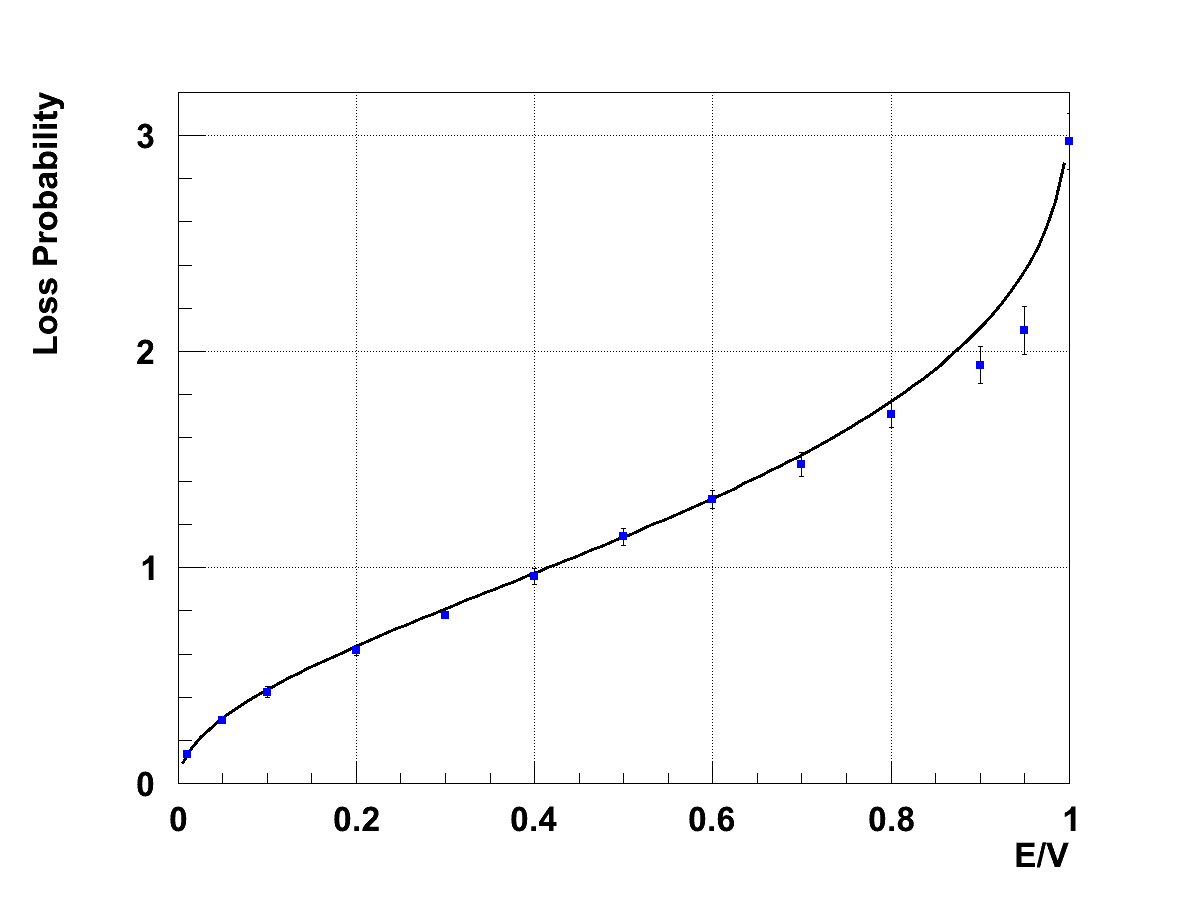
\includegraphics[scale=0.3]{figures/LossFunction-1000}
\end{center}
\caption{Angle-averaged Loss probability as a function of neutron energy}
\label{fig:NestedBox}
\end{figure}

\subsection{Monte-Carlo Test against Angle-averaged Loss Probability Curve}

In the simulation, we used a simple cylinder (dimensions relevant to a later test, radius = 0.235m, height = 0.12m), orientated vertically with respect to a gravitational field along the z-axis. To simulate losses at a boundary, we first made an implementation of a realistic material for the surfaces of the cylinder, using the following approach, \cite{Pe.09}.

Neutrons in a given material bottle will have a lifetime $\tau$ shorter than the beta-decay lifetime, and depends on the losses from interaction with the material walls. Now it is clear that, the number of collisions with the wall in the lifetime $\tau$, multiplied by the probability of loss per collision, will equal one. 

\begin{equation}
(N_{c} \tau) \times \bar{\mu}(E) = 1
\label{eqn:collisionsintau}
\end{equation}

where, $N_{c}$ represents the number of collisions per second. The number of collisions per second $N_{c}$ can be calculated using the mean free path between collisions for an isotropic gas, $\lambda$, a result from classical statistical physics giving,

\begin{equation}
(\frac{v}{\lambda} \tau) \times 2f \left[ \frac{V}{E} \arcsin \left( \frac{E}{V} \right) ^{\frac{1}{2}} - \left(\frac{V}{E} - 1 \right)^{\frac{1}{2}} \right] = 1
\label{eqn:meanfreepathcollisionsintau}
\end{equation}

where, $v$ is the average neutron velocity. 

[ For full derivation, I've included a subsection on this result. This needs to be worked into the main text. ]

\subsection*{Calculating the Rate of Loss at the Boundary}

To calculate the rate of loss of neutrons from the boundary, we need to know the rate of neutrons colliding with the surface of the volume per unit time, per unit surface area. 

For neutrons in the UCN energy regime, their interactions are such that they can effectively be modelled as an isotropic, UCN `gas', since they effectively do not interact with each other or the liquid helium medium that surrounds them. In this case, the classical results from kinetic theory for the motions of molecules in a ideal gas can be applied to UCN in certain cases with some success. 

Consider first, the one-dimensional case from classical kinetic theory. 

Imagine a portion of the wall of surface area $A$, and a neutron which hits the surface with velocity in the x-direction, $v_{x}$. In a time $\Delta t$ the molecule will travel a distance $v_{x} \Delta t$ in the positive x-direction, if $v_{x}$ is positive. The neutron will hit the wall if the distance to the wall is less than this distance $v_{x} \Delta t$, so there is a volume, $A v_{x} \Delta t$, in which any neutron with velocity $v_{x}$ in the positive x-direction will hit the wall. 

Now the number density of neutrons in this volume, is just $N/V$, assuming the neutrons are uniformly distributed, which is usually the case (except near the source or detector!), so this small volume contains, 

\begin{equation}
	\mbox{Number of particles within reach of the wall} = \frac{N}{V}Av_{x}\Delta t
\end{equation} 

neutrons. The number of these neutrons with velocity $v_{x}$, is the number of neutrons within this slab of volume, multiplied by the number with velocity $v_{x}$, which is usually given by the Maxwell-Boltzmann distribution, $f(v_{x})$,

\begin{equation}
\mbox{Number of neutrons in slab with velocity } v_{x} = \frac{N}{V}Av_{x}\Delta t f(v_{x})\mathrm{d}v_{x}
\end{equation}

The total number of collisions is then just the integrating this expression over the positive velocities, 

\begin{equation}
\frac{N}{V}A\Delta t \int_{0}^{\infty} v_{x}f(v_{x})\mathrm{d}v_{x} = \frac{N}{V}A\Delta t . \, \frac{1}{2}\left( \int_{-\infty}^{\infty} |v_{x}|f(v_{x})\mathrm{d}v_{x} \right) = \frac{N}{V}A\Delta t \frac{\langle |v_{x}| \rangle}{2}
\end{equation}

where we have used the fact that $|v_{x}|f(v_{x})$ is an even function of $v_{x}$ (i.e: $f(v_{x}) \propto v_{x}^{2}e^{-v^{2}_{x}}$), and used the definition of the average of the absolute value of $v_{x}$,

\begin{equation}
\langle |v_{x}| \rangle \equiv \int_{-\infty}^{\infty} |v_{x}|f(v_{x})\mathrm{d}v_{x}
\end{equation}

Therefore, the number of collisions per unit time, per unit area, is obtained by dividing the above total number of collistions, by the area of the collision surface, $A$ and by the time interval $\Delta t$, 

\begin{equation}
\mbox{Number of collisions per unit time \& area} = \frac{1}{2}\frac{N}{V} \langle |v_{x}| \rangle
\label{eqn:numbercollisionsperunitareatime}
\end{equation}

Now, the typical form of the one-dimensional maxwell-boltzmann distribution is, 

\begin{equation}
f(v_{i}) = \sqrt{\frac{m}{2\pi k T}} e^{-\frac{mv_{i}^{2}}{2kT}}
\end{equation}

If we evaluate the integral defined above for $\langle |v_{x}| \rangle$, we get,

\begin{eqnarray*}
\langle |v_{x}| \rangle &\equiv& \int_{-\infty}^{\infty} |v_{x}|f(v_{x})\mathrm{d}v_{x} \\
&=& 2\int_{0}^{\infty} v_{x} \sqrt{\frac{m}{2\pi k T}} e^{-\frac{mv_{i}^{2}}{2kT}}  dv_{x} \\
\end{eqnarray*}

which can be solved using the substitution $\frac{mv_{x}^{2}}{2kT} = u$, 

\begin{eqnarray*}
\langle |v_{x}| \rangle &\Rightarrow& \sqrt{\frac{2kT}{\pi m}} \int_{0}^{\infty} e^{-u} du \\
&=& \sqrt{\frac{2kT}{\pi m}} -\left[e^{-\infty} - e^{0}\right] \\
&=& \sqrt{\frac{2kT}{\pi m}}
\end{eqnarray*}

Now we would like to generalise this result to three dimensions, for which the maxwell-boltzmann distribution becomes, 

\begin{equation}
f(v) = 4\pi \left(\frac{m}{2\pi k T}\right)^{\frac{3}{2}} v^{2} e^{-\frac{mv^{2}}{2kT}}
\end{equation}

where here, $v = \sqrt{v_{x}^{2} + v_{y}^{2} + v_{z}^{2}}$.

Analogous to the case for $v_{x}$ above, we can calculate the average speed, 

\begin{equation}
\langle v \rangle \equiv \int_{0}^{\infty} vf(v) dv =  4\pi \left(\frac{m}{2\pi k T}\right)^{\frac{3}{2}} \int_{0}^{\infty} v^{3} e^{-\frac{mv^{2}}{2kT}} dv
\end{equation}

which can be solved analytically as well, (although requires a bit more work!). The general result is, 

\begin{equation}
\int_{0}^{\infty} x^{3} e^{-ax^{2}} dx = \frac{1}{2a^{2}}
\end{equation}

therefore, 

\begin{eqnarray*}
\langle v \rangle &=& 4\pi \left(\frac{m}{2\pi k T}\right)^{\frac{3}{2}} \times \frac{1}{2(\frac{m}{2kT})^{2}} \\
&=& 8\pi \left(\frac{m}{2\pi k T}\right)^{\frac{3}{2}}\left( \frac{kT}{m} \right)^{2} \\
&=& \sqrt{\frac{8kT}{\pi m}} \\
&=& 2 \langle |v_{x}| \rangle 
\end{eqnarray*}

where in the last step we used the result from above, 

\begin{equation}
\langle |v_{x}| \rangle = \sqrt{\frac{2kT}{\pi m}} = \frac{1}{2}\sqrt{\frac{8kT}{\pi m}}
\end{equation}

Thus, we can finally go back to equation \ref{eqn:numbercollisionsperunitareatime}, and write, 

\begin{eqnarray*}
\mbox{Number of collisions per unit time \& area} &=& \frac{1}{2}\frac{N}{V} \langle |v_{x}| \rangle \\
&=& \frac{1}{4}\frac{N}{V}\langle v \rangle
\end{eqnarray*}

Finally now, we can calculate the rate of loss, $\Gamma$, at a particular boundary with surface area $A$, :

\begin{equation}
\Gamma = \frac{1}{4}\frac{N}{V}A\langle v \rangle \times \bar{\mu}(E)
\end{equation}

where, we have introduced $\bar{\mu}(E)$, which is the probability of loss at a boundary, averaged over all angles of incidence. The derivation for this is given in another section. 

%%%%%%

Using the above, we can calculate a value for $f$, and hence the imaginary part of the potential $W$, which we can then use in the simulation to calculate the probability of loss at every collision. Using some experimentally determined values from the room-temperature EDM experiment, \cite{Pe.09}, that again, are more relevant to a later test but still of course applicable now, we can extract a value for $f$:
\begin{eqnarray*}
\bar{v} &=& \mbox{average particle velocity} = 3.2 \mbox{m/s} \\
\lambda &=& \mbox{mean free path} = \frac{4V}{A_{walls} + A_{ends}} = \frac{2RH}{H+R} = 0.159 \mbox{m.  For $R = 0.235$m, $H = 0.12$m} \\
V &=& \mbox{Fermi potential of walls, assumed to be quartz} = 93.3 \mbox{neV.    (0.91m in height equivalent units)} \\
E &=& \mbox{UCN energy at 3.2m/s} = 53.3 \mbox{neV.     (0.52m in height equivalent units)} \\
\Rightarrow f &=& 2.63\times10^{-4}
\end{eqnarray*}

Now, in the simulation we create a cylinder with walls made from a material with the above Fermi potential, $V$, and $f$, and then use equation \ref{eqn:lossprobabilityperbounce} to calculate the loss probability at that specific angle of incidence $\theta$ and \textbf{kinetic} energy at the collision, $E$. Finally, we use a random number generator to determine whether a loss occurred. Every run of the simulation uses an initial distribution of neutrons that are spread uniformly throughout the cylinder, and given a random starting direction that is uniformly distributed about a sphere. Their starting \textbf{total} energy is the same everywhere, which is of course the kinetic plus gravitational potential energy. This value is defined at the zero of the gravitational potential - the bottom of the cylinder - and will normally be quoted as a fraction of the Fermi-potential $E_{T}/V$.

We run the simulation until all of the neutrons have been lost to the boundary (ignoring beta-decay in this instance). We then bin the number of collisions made by each neutron before it was lost to the boundary and fit the resulting histogram to an exponential as shown in figure \ref{fig:collisionbeforeloss}. 

\begin{figure}[!htbp] 	
\begin{center}
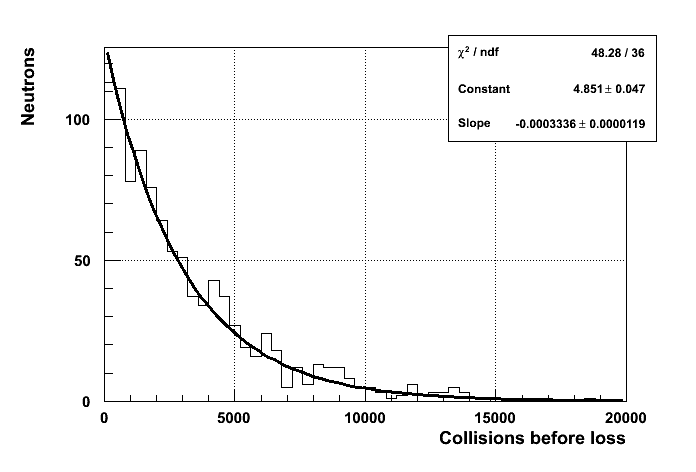
\includegraphics[scale=0.5]{figures/collisionsbeforeloss-0_57EV}
\end{center}
\caption{Number of collisions made by the neutrons before being lost to the material boundary, for a starting total energy of 0.57E/V}
\label{fig:collisionbeforeloss}
\end{figure}

From the fitted exponential exp$(-t/\tau)$, we can extract a value for $\tau$, the bottle lifetime, and therefore a value for the `angle-averaged' probability of loss $\bar{\mu}(E) = 1/\tau(E)$ for that particular starting energy, which we can compare against the expected value from equation \ref{eqn:angleaveragedlossprobability}.

Running our simulation over a range of starting energies in the above manner, produces figure \ref{fig:simulatedangleavragedlossprob}, which shows the simulated values of the loss probability drawn beside the analytical curve.

\begin{figure}[!htbp] 	
\begin{center}
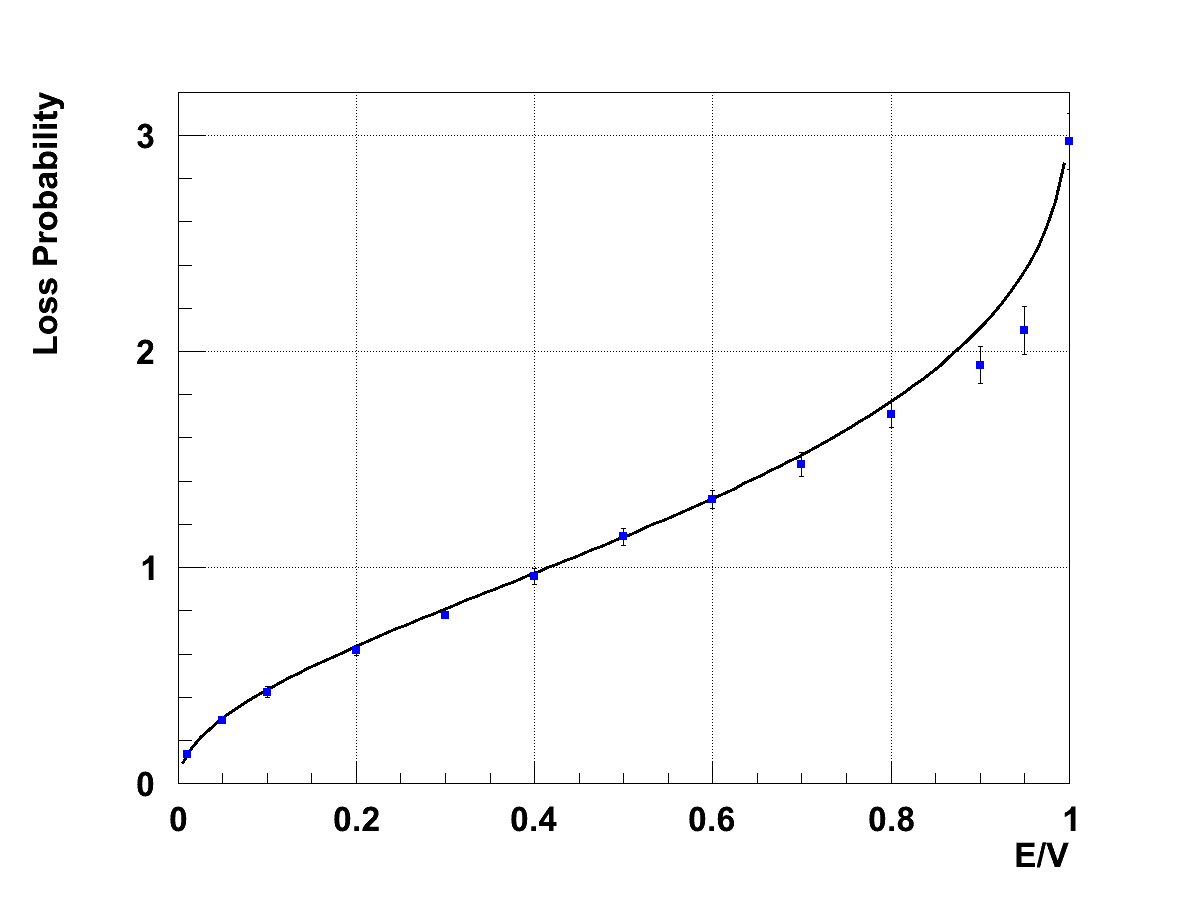
\includegraphics[scale=0.3]{figures/LossFunction-1000}
\end{center}
\caption{Plot of the simulated values for the angle-averaged Loss probability as a function of neutron energy, drawn beside the expected curve from the analytical expression in equation \ref{eqn:angleaveragedlossprobability}}
\label{fig:simulatedangleavragedlossprob}
\end{figure}

From figure \ref{fig:simulatedangleavragedlossprob}, the simulated values begin to diverge from the analytical curve at around 0.8 E/V, and gets worse the higher energy you go to. At this energy, it was thought that the angular distribution of the neutrons might not be staying uniform, as the high energy will lead to those neutrons approaching the boundary at angles close to its normal direction, will be lost very rapidly, and thus without a significant amount of diffuse scattering, angular uniformity would be lost. Preliminary tests of this hypothesis, by varying the proportion of diffuse scattering for a particular energy, did not significantly alter this divergence from the analytical curve however. 

[ Still need to add this plot to the document ]

\subsection*{Simulation Test Outcome}

\begin{itemize}
\item  Fit to analytical curve is very good up until the high energy range $>$ 0.8 E/V, therefore no major problems with simulation are believed to be present in this area.
\item  High energy range needs further investigation, such as reproducing the fit's dependence on diffuse scattering proportion. 
\end{itemize}


\section{Volume-Averaged Magnetic Field Calculation}

Another test using the exact same set-up as the angle-averaged loss probability test, is to calculate the volume-averaged magnetic field, for a particular magnetic field, by calculating the average magnetic field seen by each neutron in the simulation as it propagates around the cylinder. The purpose of the test is to determine how the influence of neutron losses at the boundary affect the result obtained - since neutron losses depend on the angle of approach to the boundary, losses will occur more frequently for those neutrons travelling through the centre of the cylinder, than those that `skim' around the edges of the cylinder. Depending on the type of magnetic field in the cylinder, this could mean that when losses are present, the volume-averaged field will be affected, as certain trajectories have a higher change of leading to the loss of that neutron. 

The magnetic field used for this test is a rotationally-symmetric field about the z-axis, that falls away parabolically with radial distance from the z-axis.
\begin{equation}
B(r,z) = B_{0} - \alpha \frac{r^{2}}{R^{2}} 
\label{eqn:magfield}
\end{equation}

where $R$, is the radius of the cylinder, $alpha$ is a numerical factor that describes how quickly the field decays away at the boundaries, and $B_{0}$ is the maximum field along the z-axis.

For our simulation, we used a value of $B_{0} = 1$ and $\alpha = 0.1$ to give a $10\%$ decay at the boundary. The analytic value for the volume-averaged magnetic field, in this case, for no neutron losses, is,
\begin{eqnarray*}
B_{avg} &=& \frac{\iiint_{V} B(r,z) \, r\mathrm{d}r\mathrm{d}\theta \mathrm{d}z }{\iiint_{V}\mathrm{d}V} \\
 &=& \frac{2}{R^{2}} \left[ \frac{1}{2}B_{0}r^{2} - \frac{1}{4}\frac{\alpha}{R^{2}}r^{4}  \right]^{R}_{0} \\
 &=& B_{0} - \frac{1}{2}\alpha \\
 &=& 0.95
\end{eqnarray*}

To make a calculation of this value within the simulation we need to calculate the integrated magnetic field along a particular path. The fact that the field does not vary with height $z$, simplifies this greatly, since, 

\begin{equation}
B(r,z) = B_{0} - \alpha \frac{r^{2}}{R^{2}} = B_{0} - \frac{\alpha}{R^{2}}(x^{2} + y^{2})
\label{eqn:magfieldcomponents}
\end{equation}

and thus, we can express the field as a function of time using the equations of motion for our particle, $x_{i}(t) = x_{i}(0) + v_{i}(0)t$ (or can also use the more general, $x_{i}(t) = x_{i}(0) + v_{i}(0)t + \frac{1}{2}g\hat{G_{i}}t^{2}$, if you needed to include a rotated cylinder),

\begin{equation}
B(t) = B_{0} - \alpha(x_{0}^{2} + y_{0}^{2}) - 2\alpha(x_{0}v_{x} + y_{0}v_{y})t - \alpha(v_{x}^{2} + v_{y}^{2})t^{2}
\label{eqn:magfieldparametric}
\end{equation}

which we can integrate over a particular trajectory, to provide the time-averaged magnetic field in this case,

\begin{equation}
B_{avg} = \frac{\int_{0}^{t} B(t) \mathrm{d}t}{t_{step}} = \frac{1}{t_{step}}\left[ B_{0}t - \alpha(x_{0}^{2} + y_{0}^{2})t - \alpha(x_{0}v_{x} + y_{0}v_{y})t^{2} - \frac{\alpha}{3}(v_{x}^{2} + v_{y}^{2})t^{3} \right]^{t_{step}}_{0}
\label{eqn:magfieldparametric}
\end{equation}

By taking the arithmetic mean of these time-averaged values for the average field over the entire neutron trajectory, we get a value for the average magnetic field seen by this neutron along its entire journey. If we do this for a large number of neutrons and take the mean of all their average sampled magnetic field, we should get an estimate of the `true' volume-averaged magnetic field. 

\subsection{Monte-Carlo Test of Volume-Averaged Magnetic Field}

For the simulation setup, we used the exact same cylinder as before ($R = 0.235$m, $H = 0.12$m), with the same value for the fermi-potential, $V = 0.91$m, and $f = 2.63\times10^{-4}$ in the cases where neutron losses were included. An element of diffuse scattering is also present in bounces to preserve the angular uniformity. This is currently a fixed percentage of bounces - 10\% - determined by a simple roll of the random number generator before every bounce. 

For an initial neutron energy (again, taken from the bottom of the cylinder at the zero of the gravitational potential) of $0.57$E/V, and with diffuse scattering turned off, the simulation produces a value for the volume-averaged magnetic field of 0.94 (figure \ref{fig:avgmagfieldnolosses}).

\begin{figure}[!htbp] 	
\begin{center}
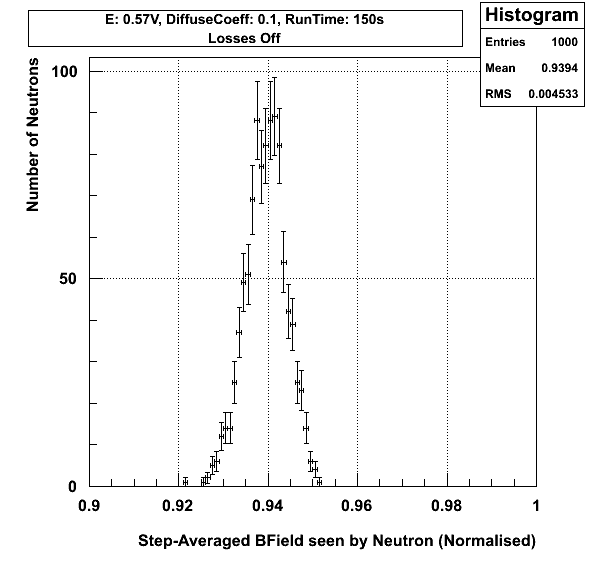
\includegraphics[scale=0.5]{figures/magfield-0_01Diff-lossesoff}
\end{center}
\caption{Plot of the average magnetic field sampled by each neutron along their entire trajectory. No losses at the boundary are present.}
\label{fig:avgmagfieldnolosses}
\end{figure}

In this case, we would expect the value to be that from the analytic calculation above that gives 0.95 as the volume-averaged magnetic field. If we now turn neutron losses at the boundary on again, and throw away those neutrons that are lost, we get the same value of 0.94.

\begin{figure}[!htbp] 	
\begin{center}
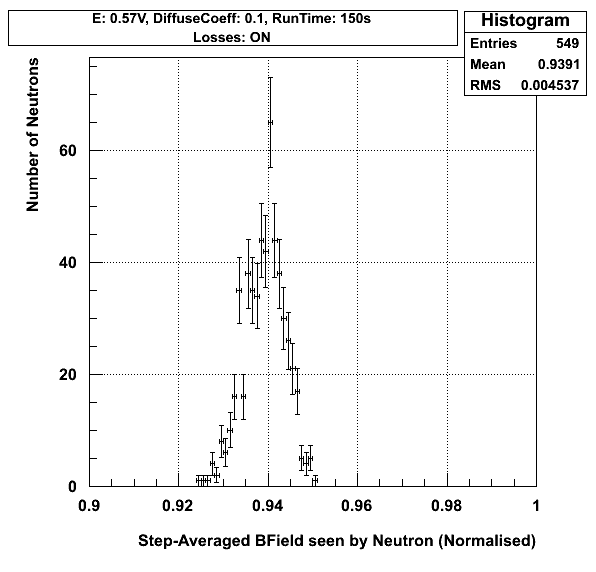
\includegraphics[scale=0.5]{figures/magfield-0_01Diff-losseson}
\end{center}
\caption{Plot of the average magnetic field sampled by each neutron along their entire trajectory. Losses at the boundary are present.}
\label{fig:avgmagfieldnolosses}
\end{figure}

These results are not what we expect to see from this test, and therefore further work must be made to understand what is causing the discrepancy in the simulation. 

\subsection*{Simulation Test Outcome}
\begin{itemize}
\item  Value for the volume-averaged magnetic field when no losses are present is a clear warning sign that the simulation is not quite right in this calculation and needs further investigation to determine what is going wrong.
\item  We also expect to see the value for the volume-averaged magnetic field when losses \textbf{are} present be lower than when losses are not present. This is currently not the case.
\end{itemize}

\pagebreak 

\begin{thebibliography}{99}
\bibitem{Go.Ri.La.91} R. Golub, Lamaroux... ``Ultra-Cold neutrons''
\bibitem{Go.Pe.79} R. Golub, J.M. Pendlebury, ``Ultra-Cold neutrons'', \emph{Rep. Prog. Phys.},	\textbf{42}, 439-501, (1979).
\bibitem{Pe.09} Private correspondence with J.M. Pendlebury
\end{thebibliography}

\end{document}